\section{Results}\label{sec:results}

% describe data
We apply our method to a set of mock data, the spherical models
for the Gaia challenge by Walker and Penarrubia. They consist of
dynamical tracer populations with density distribution

\begin{equation}
    \nu_*(r) = \nu_0\left(\frac{r}{r_*}\right)^{-\gamma_*} \left[1+\left(\frac{r}{r_*}\right)^{\alpha_*}\right]^{(\gamma_*-\beta_*)/\alpha_*}
\end{equation}

inside dark matter halos of the form

\begin{equation}
    \rho_{\text{DM}} = \rho_0\left(\frac{r}{r_{\text{DM}}}\right)^{-\gamma_{\text{DM}}}\left[1+\left(\frac{r}{r_{\text{DM}}}\right)^{\alpha_{\text{DM}}}\right]^{(\gamma_{\text{DM}}-\beta_{\text{DM}})/\alpha_{\text{DM}}}
\end{equation}

with scale radii $r_*, r_\text{DM}$, inner and outer logarithmic
slopes of $\gamma_*, \gamma_{\text{DM}}$ and
$\beta_*,\beta_{\text{DM}}$, with transition parameters $\alpha_*,
\alpha_{\text{DM}}$.

The anisotropy follows the functional form of \citet{Osipkov1979} and
\citet{Merritt1985},

\begin{equation}
    \beta_{\text{anisotropy}}(r)=1-\frac{\sigma_\theta^2}{\sigma_r^2} = \frac{r^2}{r^2+r_a^2}.
\end{equation}

with scale radius $r_a$, turning over from nearly isotropic at $r\to
0$ to radially biased at $r_*=r_a$.

Of these distributions, finite samplings are taken and converted to
mock observational data including observational parameters like
spectral indices, systemic velocities, proper motions, and binary
motion.

\TODO{mention Gaia challenge}


\subsection{Cusps and Cores}

Applied on a profile with a cusp in the DM density profile, our method
reproduces the density profile (fig. \ref{fig:cusp}).

\begin{figure*}
    \begin{center}
        \hspace{-7mm}
        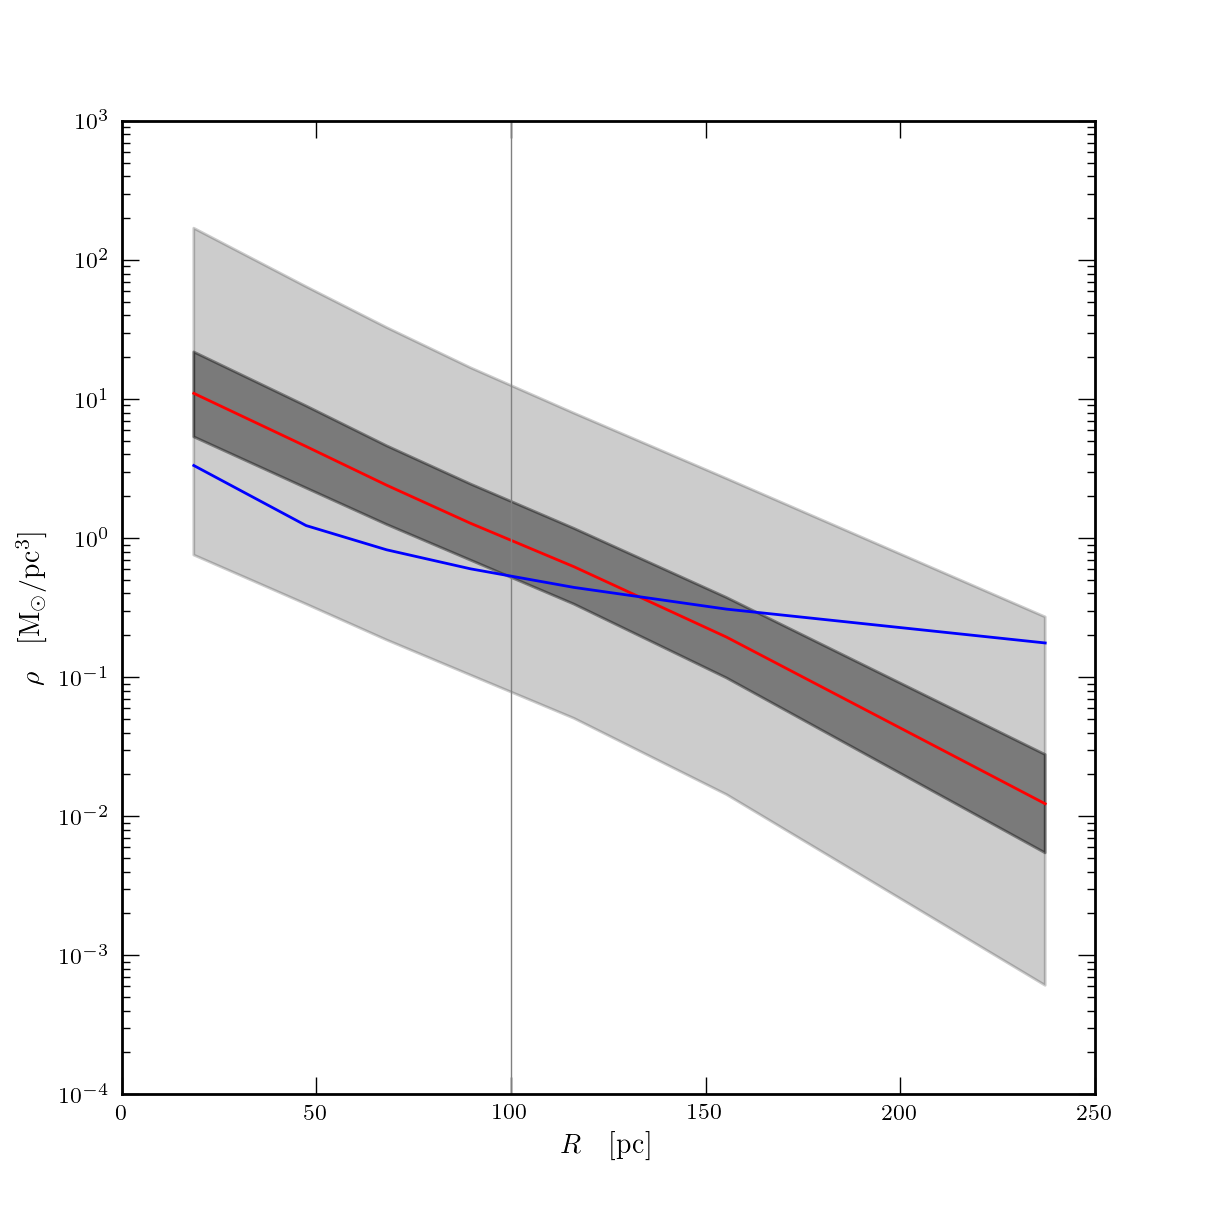
\includegraphics[width=0.3\textwidth]{fig/prof_dens.png}
        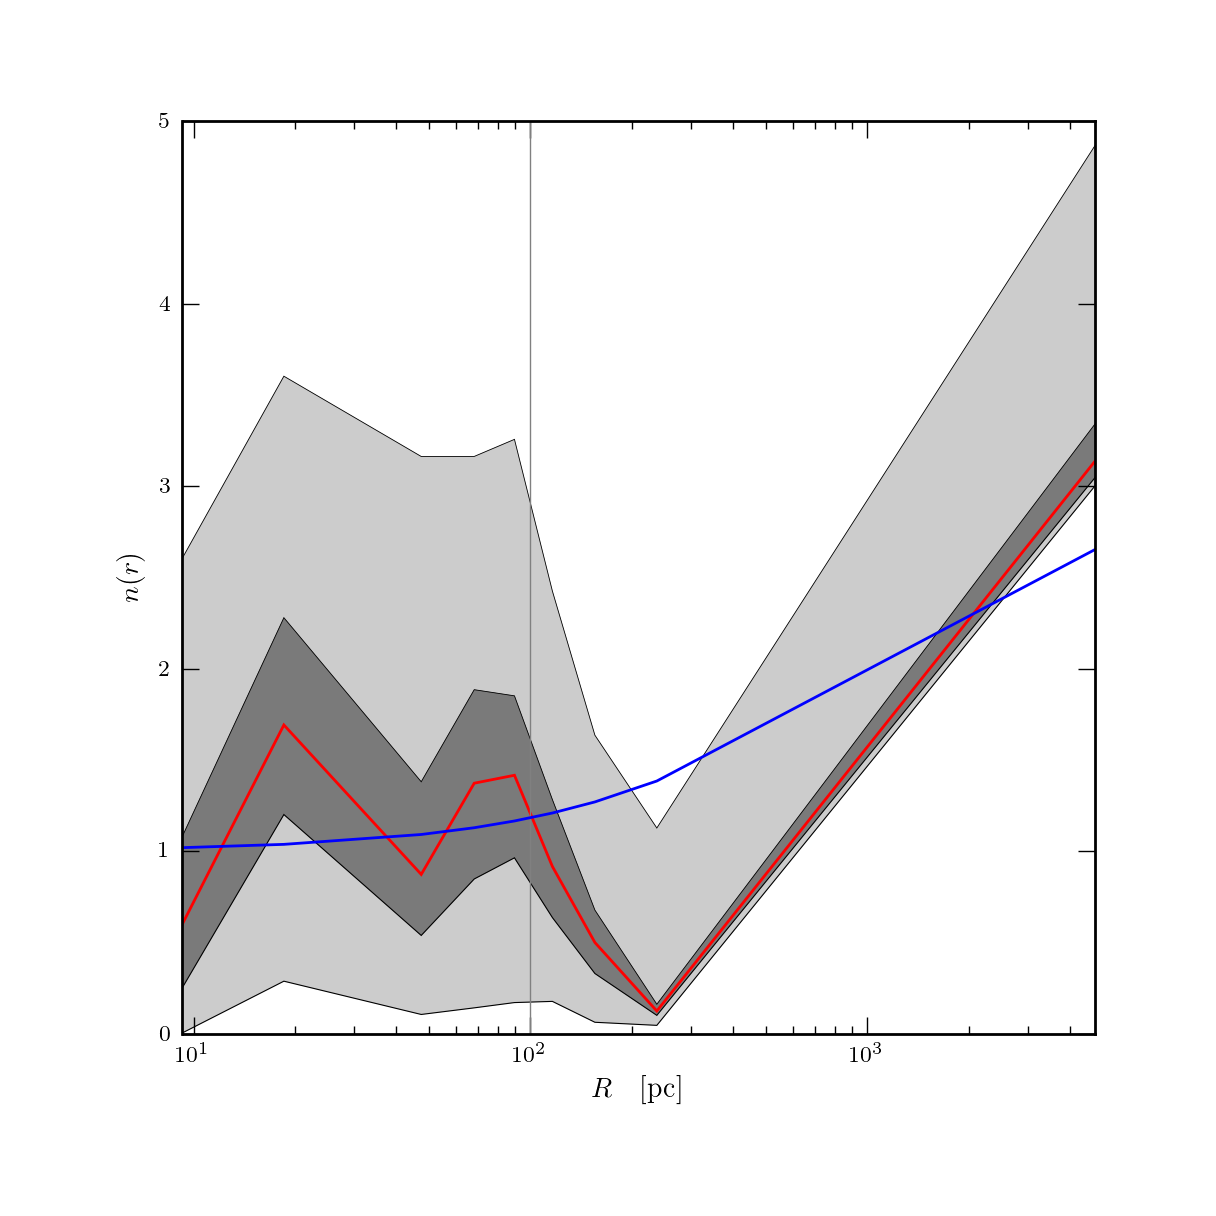
\includegraphics[width=0.3\textwidth]{fig/prof_nr.png}
        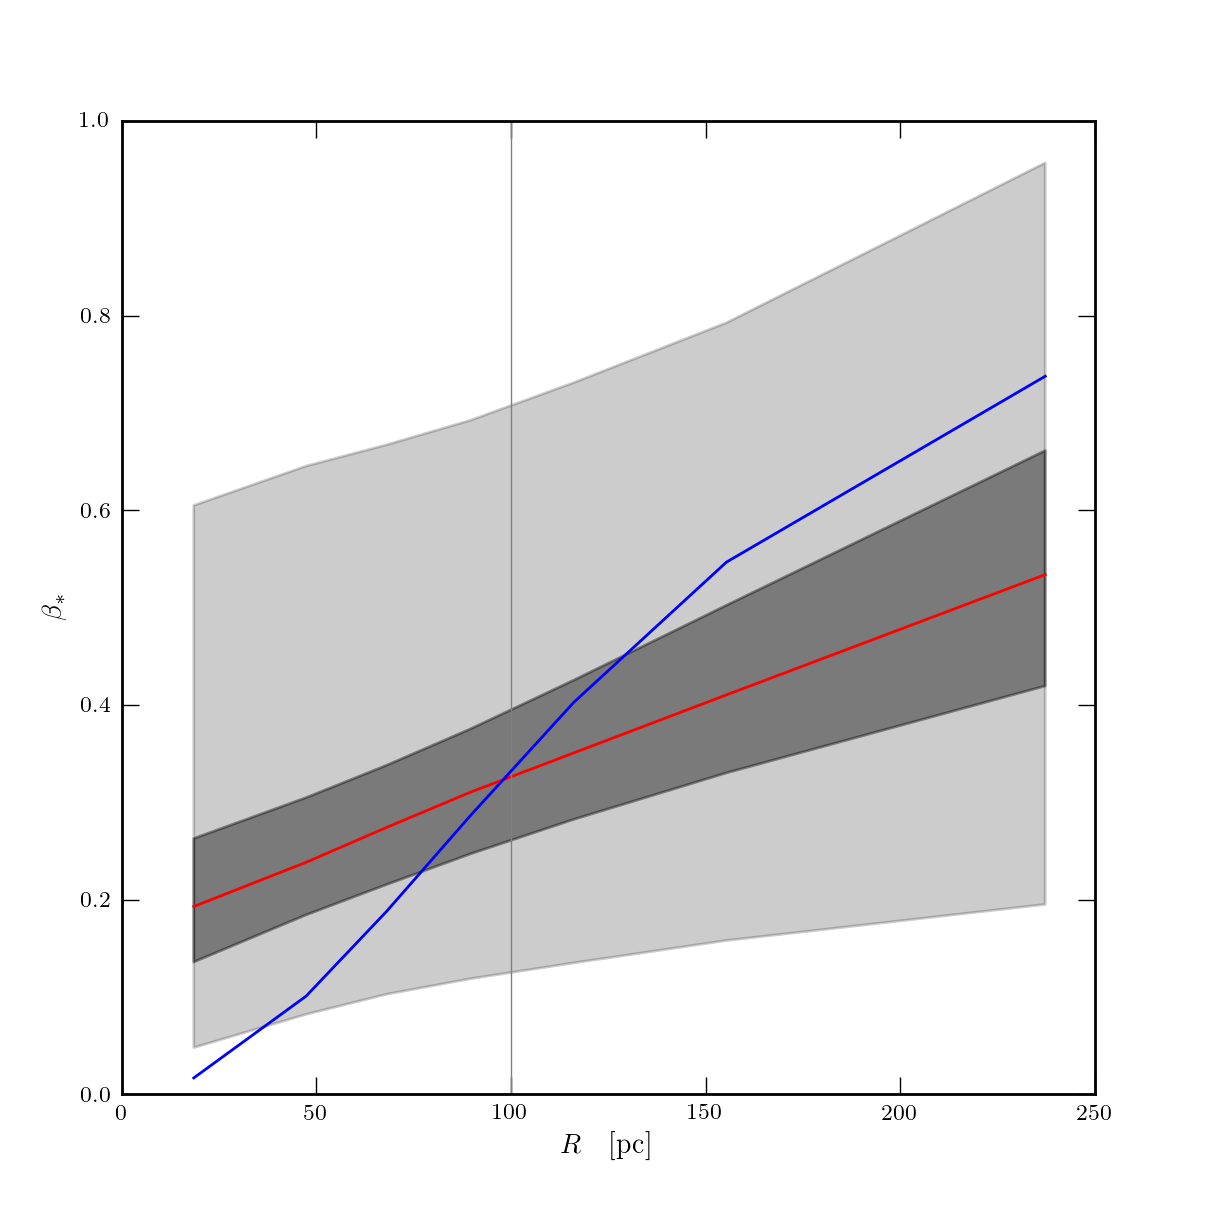
\includegraphics[width=0.3\textwidth]{fig/prof_betastar1.png}
        \caption{Reconstructed density, density slope, and velocity
          anisotropy of a cusped model (red shows median, shaded areas
          are 68 and 95 percentiles) for $10^4$ tracer particles, for
          $3\cdot10^5$ models. The blue curve shows the underlying
          theoretical model. The half-light radius of all stellar
          tracer particles is depicted as gray vertical line.}
        \label{fig:cusp}
    \end{center}
\end{figure*}


% nu and sigma: fit to data
Fitted $\nu(r)$ and $\siglos$ are shown in fig. \ref{fig:nusiglos}.

\begin{figure*}
    \begin{center}
        \hspace{-7mm}
        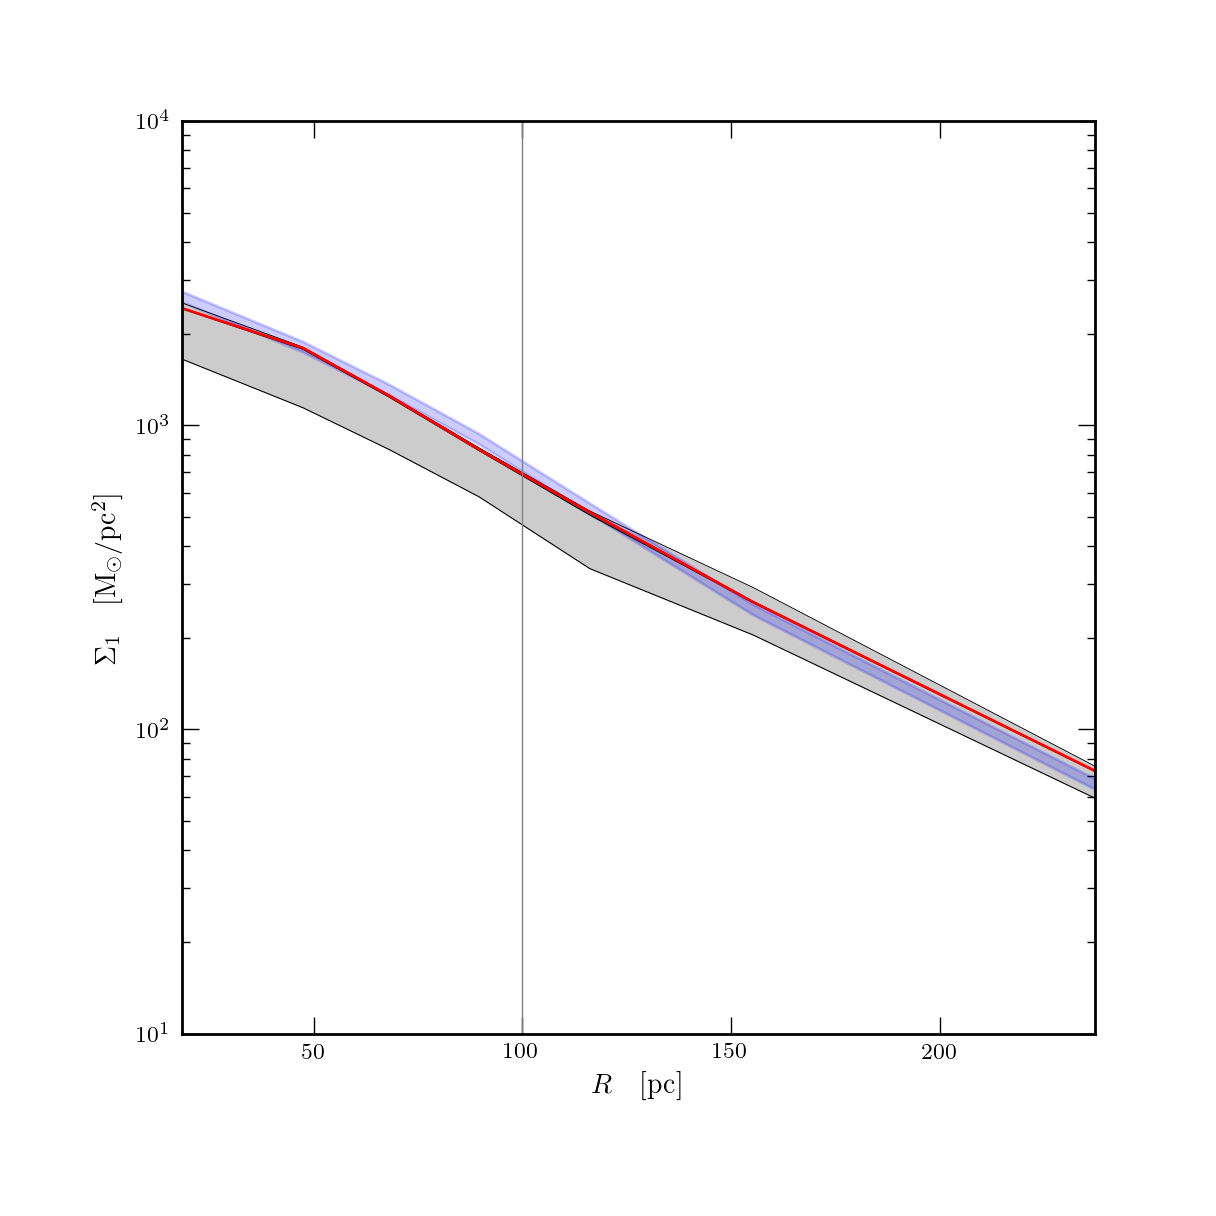
\includegraphics[width=0.5\textwidth]{fig/prof_nu.png}
%        \includegraphics[width=0.5\textwidth]{fig/prof_sig.png}
        \caption{\label{fig:nusiglos} Fitted $\nu(r)$ and $\siglos(r)$ for
          the stellar components in the cusped profile of
          fig. \ref{fig:cusp}.}
    \end{center}
\end{figure*}


% fit to underlying beta
Introducing $\kappa_i$ in the $\chi^2$ did \TODO{not?} result in a
change of behavior for the velocity anisotropy parameter.

\TODO{observations for kurtosis}
\TODO{better/worse fitting of density}


\subsection{Cored Model}
For a cored profile, we have a similar result, see fig. \ref{fig:core}. \TODO{rerun}

\begin{figure*}
    \begin{center}
        \hspace{-7mm}
        % \includegraphics[width=0.5\textwidth]{fig/.pdf}
        \caption{A cored profile: Reconstructed mass of the MCMC model
          (red shows median, shaded areas are 68 and 90 percentiles)
          for $10^4$ tracer particles based on $3\cdot10^5$ sampled
          models. The blue curve shows the underlying theoretical
          model.}
        \label{fig:core}
    \end{center}
\end{figure*}


\subsection{Triaxial mock data}
\TODO{motivation: triaxiality of observed dwarfs, effects from other
  mass modelling schemes}

The models were generated with a Made 2 Measure algorithm of
\cite{Dehnen2009} and are tailored to follow a similar profile to the
profiles specified above for the dwarf galaxies. They show a density
profile of

\begin{equation}
    \rho(r)=\frac{\rho_S}{\left(\frac{r}{r_S}\right)^\gamma\left(1+\left(\frac{r}{r_S}\right)^{1/\alpha}\right)^{\alpha(\beta-\gamma)}}
\end{equation}

with radius $r$, scale radius $r_S=1.5\kpc$, $\alpha=1$,
$\beta=4$. For the cusped profiles we have an inner logarithmic slope
of $-\gamma=-1$, scale density $\rho_S=5.522\cdot 10^7M_\odot/\kpc^3$,
and $M_{\tot}=1.171\cdot10^9M_\odot$, while for the cored one we have
$\gamma=0.23$, $\rho_S=1.177\cdot10^8M_\odot$,
$M_{\tot}=1.802\cdot10^9M_\odot$. The axis ratios are $b/a=0.8$ and
$c/a=0.6$. The stars have negligible mass and follow the same
functional form in the density profile as dark matter, with
$\alpha=0.34, \beta=5.92, \gamma=0.23, r_S=0.81\kpc$.

The velocity anisotropy of the stellar part is calculated via

\begin{equation}
\beta(r)=\frac{r_{s,\beta}^\eta \beta_0+r^\eta \beta_\infty}{r^\eta+r_{s,\beta}^\eta},
\end{equation}

with $r_{s,\beta}=0.81\kpc$, $\beta_0=0$, $\beta_\infty=0.5$ and
$\eta=0.5$, going from isotropic to radially anisotropic with
increasing radius.

\begin{figure*}
    \begin{center}
        \hspace{-7mm}
        \TODO{redo triaxial model}
        %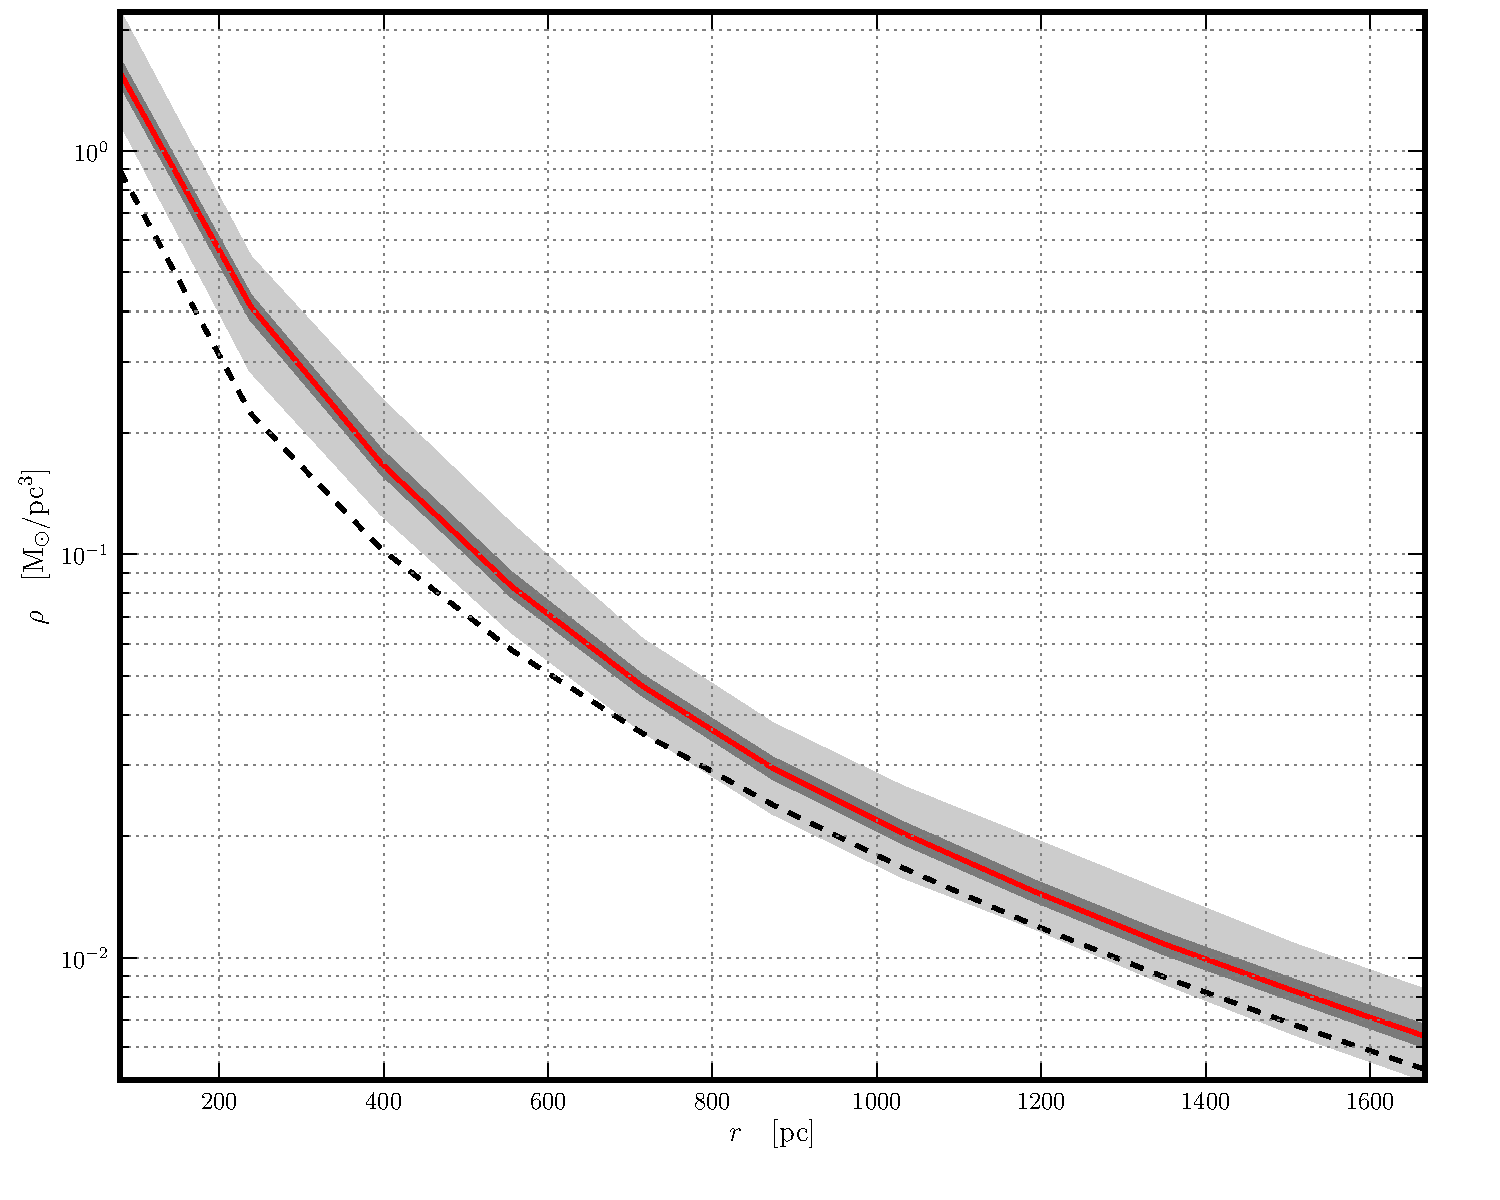
\includegraphics[width=0.5\textwidth]{fig/20130718123300_cprior_nulog_denslog_mslope_rprior_profdens.pdf}
        \caption{Density profile of a triaxial mock dwarf, for which the line
          of sight is inclined with 45 degrees with respect to all axes.}
        \label{fig:triax}
    \end{center}
\end{figure*}

The retrieved density profile (fig. \ref{fig:triax}) is constantly
overestimating the density.

\TODO{other projections}
\TODO{reason: projection}

